%\noindent Experiment N\textsuperscript{\underline{o}} Sxxx Safety Report\\
%TBA : EMMA PGAC detector test\\
%\\
\title{EMMA PGAC Detector Test\\ Safety Report}
\author{\authname\footnote{Experiment Leader/Safety Coordinator.  Tel.: +1 (604) 222-1047 x6859. \newline  \textit{\hspace*{1.5em} E-mail address:} \href{mailto:jon.lighthall@triumf.ca}{jon.lighthall@triumf.ca} (J.\ Lighthall).} \\ \small \itshape TRIUMF, 4004 Wesbrook Mall, Vancouver, BC V6T\,2A3, Canada}
\date{\small \longusdate \today}%\formatdate{24}{2}{2009}
\maketitle
%\noindent Experiment Leader/Safety Coordinator:
%\begin{changemargin}{\parindent}
%\noindent Jon Lighthall\\
%TRIUMF\\
%4004 Wesbrook Mall\\
%Vancouver, BC V6T\,2A3\\
%Canada\\
%%\href{callto:6042221047p6859}
%{(604) 222-1047 x6859}\\%+44 1904 322221\\
%\href{mailto:lighthall@triumf.ca}{lighthall@triumf.ca}\\
%%Local Contact: -Gordon Ball\\
%\end{changemargin}
\pagestyle{fancy}
\rhead{EMMA PGAC Safety Report}
\lhead{}
\renewcommand{\headrulewidth}{0pt}
%\doublespacing \linenumbers
\section{Introduction}
\subsection{Revision}
The EMMA PGAC detector was partially characterized in a similar experiment in late April, 2014. The safety report for the previous test can be found in Ref.~\cite{old_safety}. This safety report is identical to that report with two exceptions: Section~\ref{det_status} has been updated to reflect the current status of the detector; and the procedures in Section~\ref{procedures} have been revised and expanded for clarity.
\subsection{Experimental aim}
%Charles Barton has extensive experience over many years with the UK PHOENIX ECRIS charge%
%breeding ions source. He was the spokesperson for the ECRIS charge breeding experiment at%
%ISOLDE where the operating parameter space and optimization of the source occurred as part of a%
%larger European research grant into charge breeding ion sources. The capabilities and limitations of%
%this versatile and powerful charge-breeding ion source are well-understood by the group at York. 
%It is understood that a facility using this source will often deliver beams of radioactive nuclei to
%experimental stations along with some level of contaminants in the beam. Users of these facilities
%should then have the capability to selectively and sensitively tag on the isotopes of interest.

The TRIUMF Detector Group has developed %a number of detectors for use at experimental facilities
the EMMA PGAC (Parallel Grid Avalanche Counter), a device that is designed to work with the radioactive beams
delivered by ISAC-II at TRIUMF.  The PGAC detector will be a key component of the detector suite at the focal plane of the EMMA spectrometer.
EMMA, currently under construction in ISAC-II,  is a recoil mass spectrometer 
which %uses electric and magnetic dipoles to
 separates recoils of nuclear reactions from the accelerated ion beam.  The reaction recoils and the unreacted beam will be dispersed  according to their mass/charge ratio.  By separating beam-like recoils from the unreacted beam, very weak reaction channels may be studied in the presence of very high-yield background channels.  In a similar manner, beam contaminants may also be separated.  
 
In order to measure the spatial distribution of particles at the focal plane, a position sensitive detector is required.  The EMMA PGAC is designed to measure the position of particles in the $x$-$y$ plane at the EMMA focal plane. %The PGAC will also provide an essential timing signal for EMMA experiments.
  The timing reference provided by the PGAC is used to measure the recoil time-of-flight, the recoil coincidence with ejectiles detected in the target chamber, and is used to generate the trigger for the data acquisition system.
%It is also designed to be able to be an ancillary detector to the TIGRESS array and should provide the capability to identify the Z of components of the accelerated beam of radioactive ions after scattering from the experimental target.
% is a position-sensitive gas avalanche counterThis position-sensitive detector 
%In addition, the PGAC can also provide limited energy loss information, which can be used for charge identification.
Ultimately the PGAC will form the entrance to the EMMA ionization chamber, a large-acceptance Bragg detector which will be used to provide $Z$-identification of the  recoils.
 
%, and provide position information to Doppler correction the $\gamma$-rays detected by the TIGRESS array.
\subsection{Beam test}
\begin{table}[ht]
\begin{center}
\begin{tabulary}{0.5\textwidth}{R|L} 
Beamline&ISAC-I, HEBT  \\
Beam&$^{16}$O\\
Beam energy&16\,MeV (1.116\,MeV/$u$)\\
Beam intensity&6.2\,pnA or 3.9$\times10^{10}$\,pps\\
Targets& Au, $^{12}$C \\
\end{tabulary}
\end{center}
\caption{Parameters of the beam test. }
\label{beam_test}
\end{table}
The beam tests at ISAC-I aim to explore the %avalanche capability
performance of the PGAC detector under realistic experimental conditions 
 %and record the signal pulse shapes
 over a range of pressure and voltage regimes.  The goal of the current beam test is to fully characterize the detector using an updated electronics scheme and new collimating detector mask. The specific beam parameters of the test are listed in Table~\ref{beam_test}. 
 The detector will be characterized with respect to its avalanche capability and 
% The performance of the detector under multiple-hit conditions will also test the 
position reconstruction capability.  These characteristics will be assessed by measuring the timing resolution and position resolution of the detector. 
%of the detector.
The experiment will be performed in the ISAC-I experimental hall and will utilize the scattering
chamber mounted at the end of the HEBT beamline. The PGAC will be mounted on an exit port of
the scattering chamber that is at an angle of 30$^\circ$ with respect to beam direction as measured
from the center of the scattering chamber.

With a beam of $^{16}$O at 1.116\,MeV/$u$, we plan to  study the elastic %Rutherford 
scattering of beam ions off a target foil into the PGAC. The scattered beam will illuminate 60\%  of the active area of the PGAC, providing test conditions which are required to fully commission the PGAC.  The beam will be tuned through an aperture %located
on a  rotating  target wheel and monitored by a Faraday cup mounted in the 0$^\circ$ exit port of the
scattering chamber.  The feedthrough for the target wheel is located off-center of the scattering chamber, however the target wheel itself will be installed on an extension arm such that the targets will be at the center of the scattering chamber. 
During the test, the beam will be focused onto one of two targets; either a 250\,$\mu$g/cm$^2$ gold target or 253.5\,$\mu$g/cm$^2$ carbon %deuterated polyethylene (C$_2$D$_4$)$_n$
 target.  Both targets will be mounted on the target wheel. The gold foil will be used initially to provide an unambiguous spectrum.  The carbon foil may be used in the latter portion of the tests to provide a more complicated spectrum, covering a wider range of energies.

Mounted on the $30^\circ$ exit port of the scattering chamber, the %active area
anode of the first PGAC will be 685\,mm from the target wheel.  With the center of the detector located at $30^\circ$ relative to the beam, the detector will cover 23.3$^\circ$--36.7$^\circ$, subtending 20.3\,msr in the laboratory.  Given an ion drift time in the PGAC of about 2\,$\mu$s, the desired maximum count rate in the detector is 250\,kHz.  Scattering from the gold foil, this count rate corresponds to a beam rate of $3.9 \times 10^{10}$\,pps or 6.2\,pnA. %   Scattering from the carbon foil, this count rate corresponds to a beam rate of 40.8\,pnA.
%Beam rates from $1\times10^5$\,pps up to $1\times10^8$\,pps will be requested to test the detector from a few 100\,counts/s up to the expected saturation rate of $1\times10^5$\,counts/s. 
With the inclusion of the 10.16\,cm diameter beam pipe, % and the proposed mask,
the detector will cover scattering angles of 25.8$^\circ$--34.2$^\circ$, subtending 12.1\,msr or 60\% of the active detector area. With the additional inclusion of the proposed mask, the exposed area is reduced by an additional 73\%.   Thus, the expected count rate is $1.0 \times 10^5$\,cps.

\section{Hardware}
\subsection{PGAC Detector}
The EMMA PGAC is a position-sensitive, multi-wire proportional counter operating in the avalanche regime. Some of the relevant specifications of the detector are listed in Table~\ref{detector}.  Two identical PGACs have been constructed and both will be tested simultaneously in the same PGAC box during these tests.  Two detectors are required for these tests in order to provide a mutual time reference.  In addition, using two detectors allows ray-tracing of the incident particles.

\begin{table}[t]
\begin{center}
\begin{tabulary}{1.0\textwidth}{R|L} 
%\begin{tabular}{p{0.45\columnwidth}|p{0.45\columnwidth}} 
% gas properties
\raggedleft Gas (ionization media)&Isobutane\\
\raggedleft Nominal operating pressure range&$P=2$--6\,Torr\\
\raggedleft PGAC box internal volume & 12.6\,L\\
\raggedleft $0^\circ$ scattering chamber internal volume & 50\,L\\
\raggedleft Maximum quantity of isobutane in PGAC box (6\,Torr)&0.25\,g\\
\hline %window properties
\raggedleft Window material &Mylar\\
\raggedleft Nominal window thickness&1--2\,$\mu$m\\
\raggedleft Window area& 66\,mm $\times$ 166\,mm (110\,cm$^2$)\\
\raggedleft Window position (from anode)& $-36.3$\,mm\hspace{5.4em}(test)\\
&$-27.2$\,mm,  $+52.8$\,mm (focal plane)\\
\raggedleft 0.9\,$\mu$m-thick window burst pressure &24\,Torr\\
\raggedleft 2.0\,$\mu$m-thick window burst pressure &57\,Torr\\
%\raggedleft Window reverse burst pressure (SiN 30\,nm)&13<P$_\textrm{rb}$<27\,mbar\\
\hline %wire properties
\raggedleft Wire material&Gold-plated tungsten\\
\raggedleft Cathode wire diameter&25\,$\mu$m\\
\raggedleft Cathode wire pitch&1.0\,mm\\
\raggedleft Number of cathode wires&166 ($x$-direction)\\
& ~~66 ($y$-direction)\\
\raggedleft Anode wire diameter&15\,$\mu$m\\
\raggedleft Anode wire pitch&1.0\,mm\\
\raggedleft Number of anode wires &$3\times22$\\  
\raggedleft Anode-cathode gap&3.18\,mm\\
\raggedleft Energized area&60\,mm $\times$ 160\,mm (96\,cm$^2$)\\
\raggedleft Fiducial area&54\,mm $\times$ 154\,mm (83\,cm$^2$)\\
\hline %voltage properties
\raggedleft Typical cathode voltage & ~~~$V_\textrm{c}=-80$\,V\\
\raggedleft Typical anode voltage & ~~~$V_\textrm{a}=+470$\,V\\
\raggedleft Typical anode-cathode voltage &$\Delta V=550$\,V\\
\end{tabulary}
\end{center}
\caption{Characteristics of the PGAC detectors and the experimental setup. Physical specifications are given for the gas, windows, wire planes, and applied voltages. The position of the windows is given relative to the anode plane; this refers to the detector nearest the target.}
\label{detector}
\end{table}

\subsubsection{Mechanical}
Each PGAC detector is rectangular in cross section with an active area 160\,mm in the $x$-direction and 60\,mm in the $y$-direction. The anodes of the two PGACs are separated by 30\,mm in the $z$-direction. The box containing the PGACs is 41\,cm wide, square in cross section, and 10\,cm deep.
%depth and weight bout 6\,kg.
The PGAC will be filled with isobutane at a pressure of 3--6\,Torr. The 12.6\,L internal gas volume of the PGAC box will be separated from the vacuum of the 50\,L scattering chamber by a 2\,$\mu$m thick Mylar window. 

The PGAC box will be mounted to the scattering chamber at the end of the HEBT beam line at an angle of 30$^\circ$ relative to the beam line.  Fig.~\ref{schematic} includes a diagram of the experimental setup and a photograph of the scattering chamber.  The PGAC will be connected to the scattering chamber by a short beam pipe.  The length of the pipe is such that the 
entire active area of the PGAC detector will be visible to beam scattered from the target
 at the center of the scattering chamber. The beam pipe will connect directly to the front of the PGAC box via an adapter plate which houses the Mylar foil. The adapter plate is shown in Fig.~\ref{photos}.

% This short beam pipe will have a flange on one end to couple it directly to the exit port of the chamber; on the other end, a flange will couple it directly to a plate on the front of the PGAC.  %Approximately 23\% of the total PGAC detector area will be exposed to scattered beam as ray-traced from the target, through the scattering chamber and coupling pipe onto the PGAC.
%\marnote{This figure should be updated!}
\begin{figure}[ht]
\centering
%\includegraphics[width=\textwidth,height=0.4\textheight,keepaspectratio]{York_PGAC_safety_rev_11c.jpg}
\hspace{\fill}
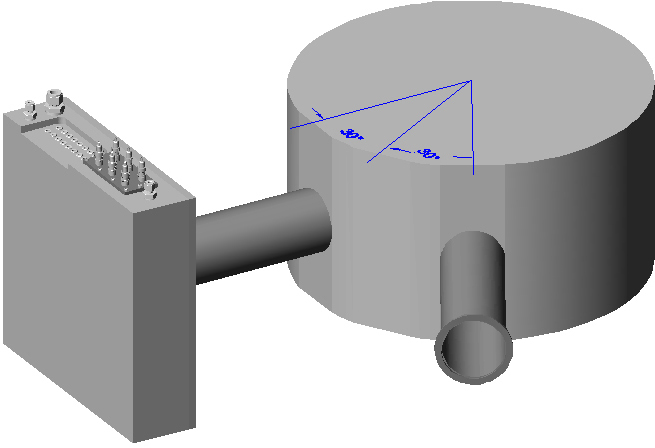
\includegraphics[width=0.48\textwidth,keepaspectratio]{HEBT_Scat_Chamber_3D_trim}\hspace{\fill}
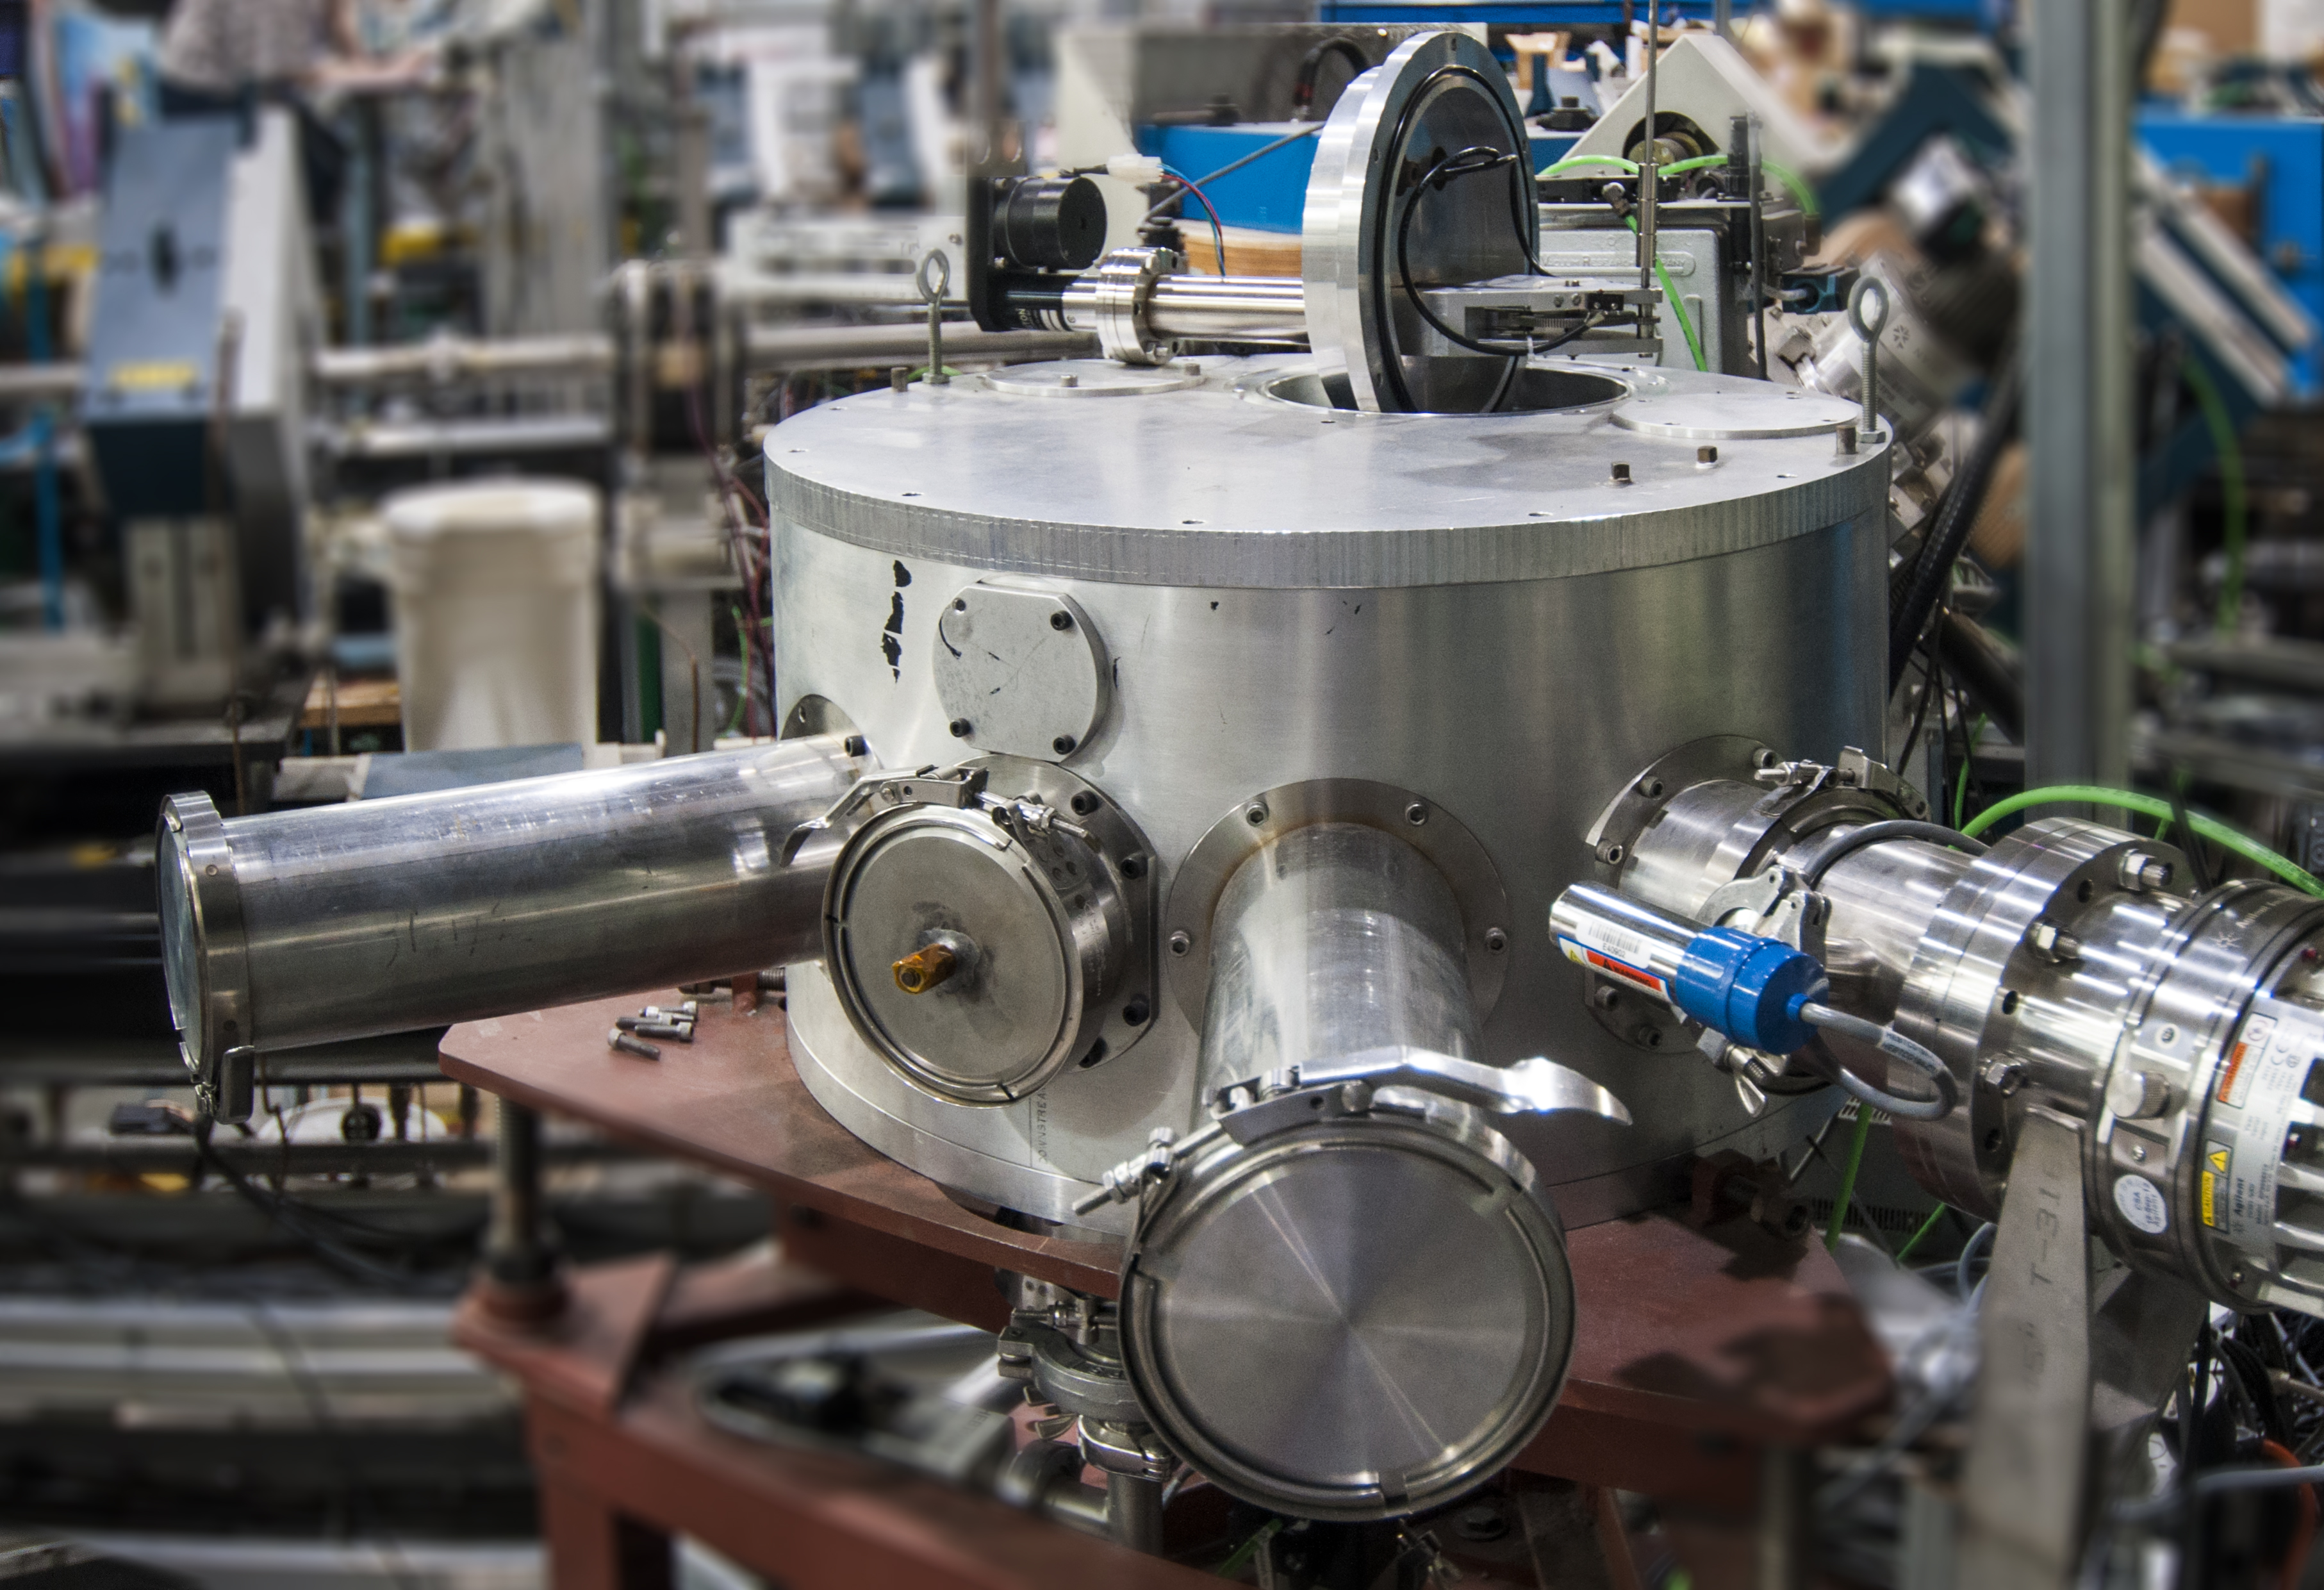
\includegraphics[width=0.48\textwidth, keepaspectratio]{DSC_0004} \hspace{\fill}
\caption{(Left) Schematic diagram of the proposed experimental setup of the 
showing a view from downstream of the HEBT beam line.  The beam enters the 0$^\circ$ scattering chamber from the top of the figure.  The beam will bombard a target foil at the center of the chamber and scattering into the PGAC box, mounted at 30$^\circ$ relative to the beam line.  The length of the beam pipe connecting the PGAC box to the scattering chamber is such that 60\% of the active area of the PGAC will be illuminated.  (Right) A photograph of the 0$^\circ$ scattering chamber before PGAC box installation.
%above %(left) and outside (right) of
%the scattering chamber. The York PGAC is shown, but the configuration of the EMMA PGAC will be similar.  The coupling flange to the PGAC, including a xx\,cm connecting pipe are shown, demonstrating the clearance of the 0$^\circ$ Faraday cup.
}
\label{schematic}
\end{figure}
\begin{figure}[ht]%
\centering
\hspace{\fill}
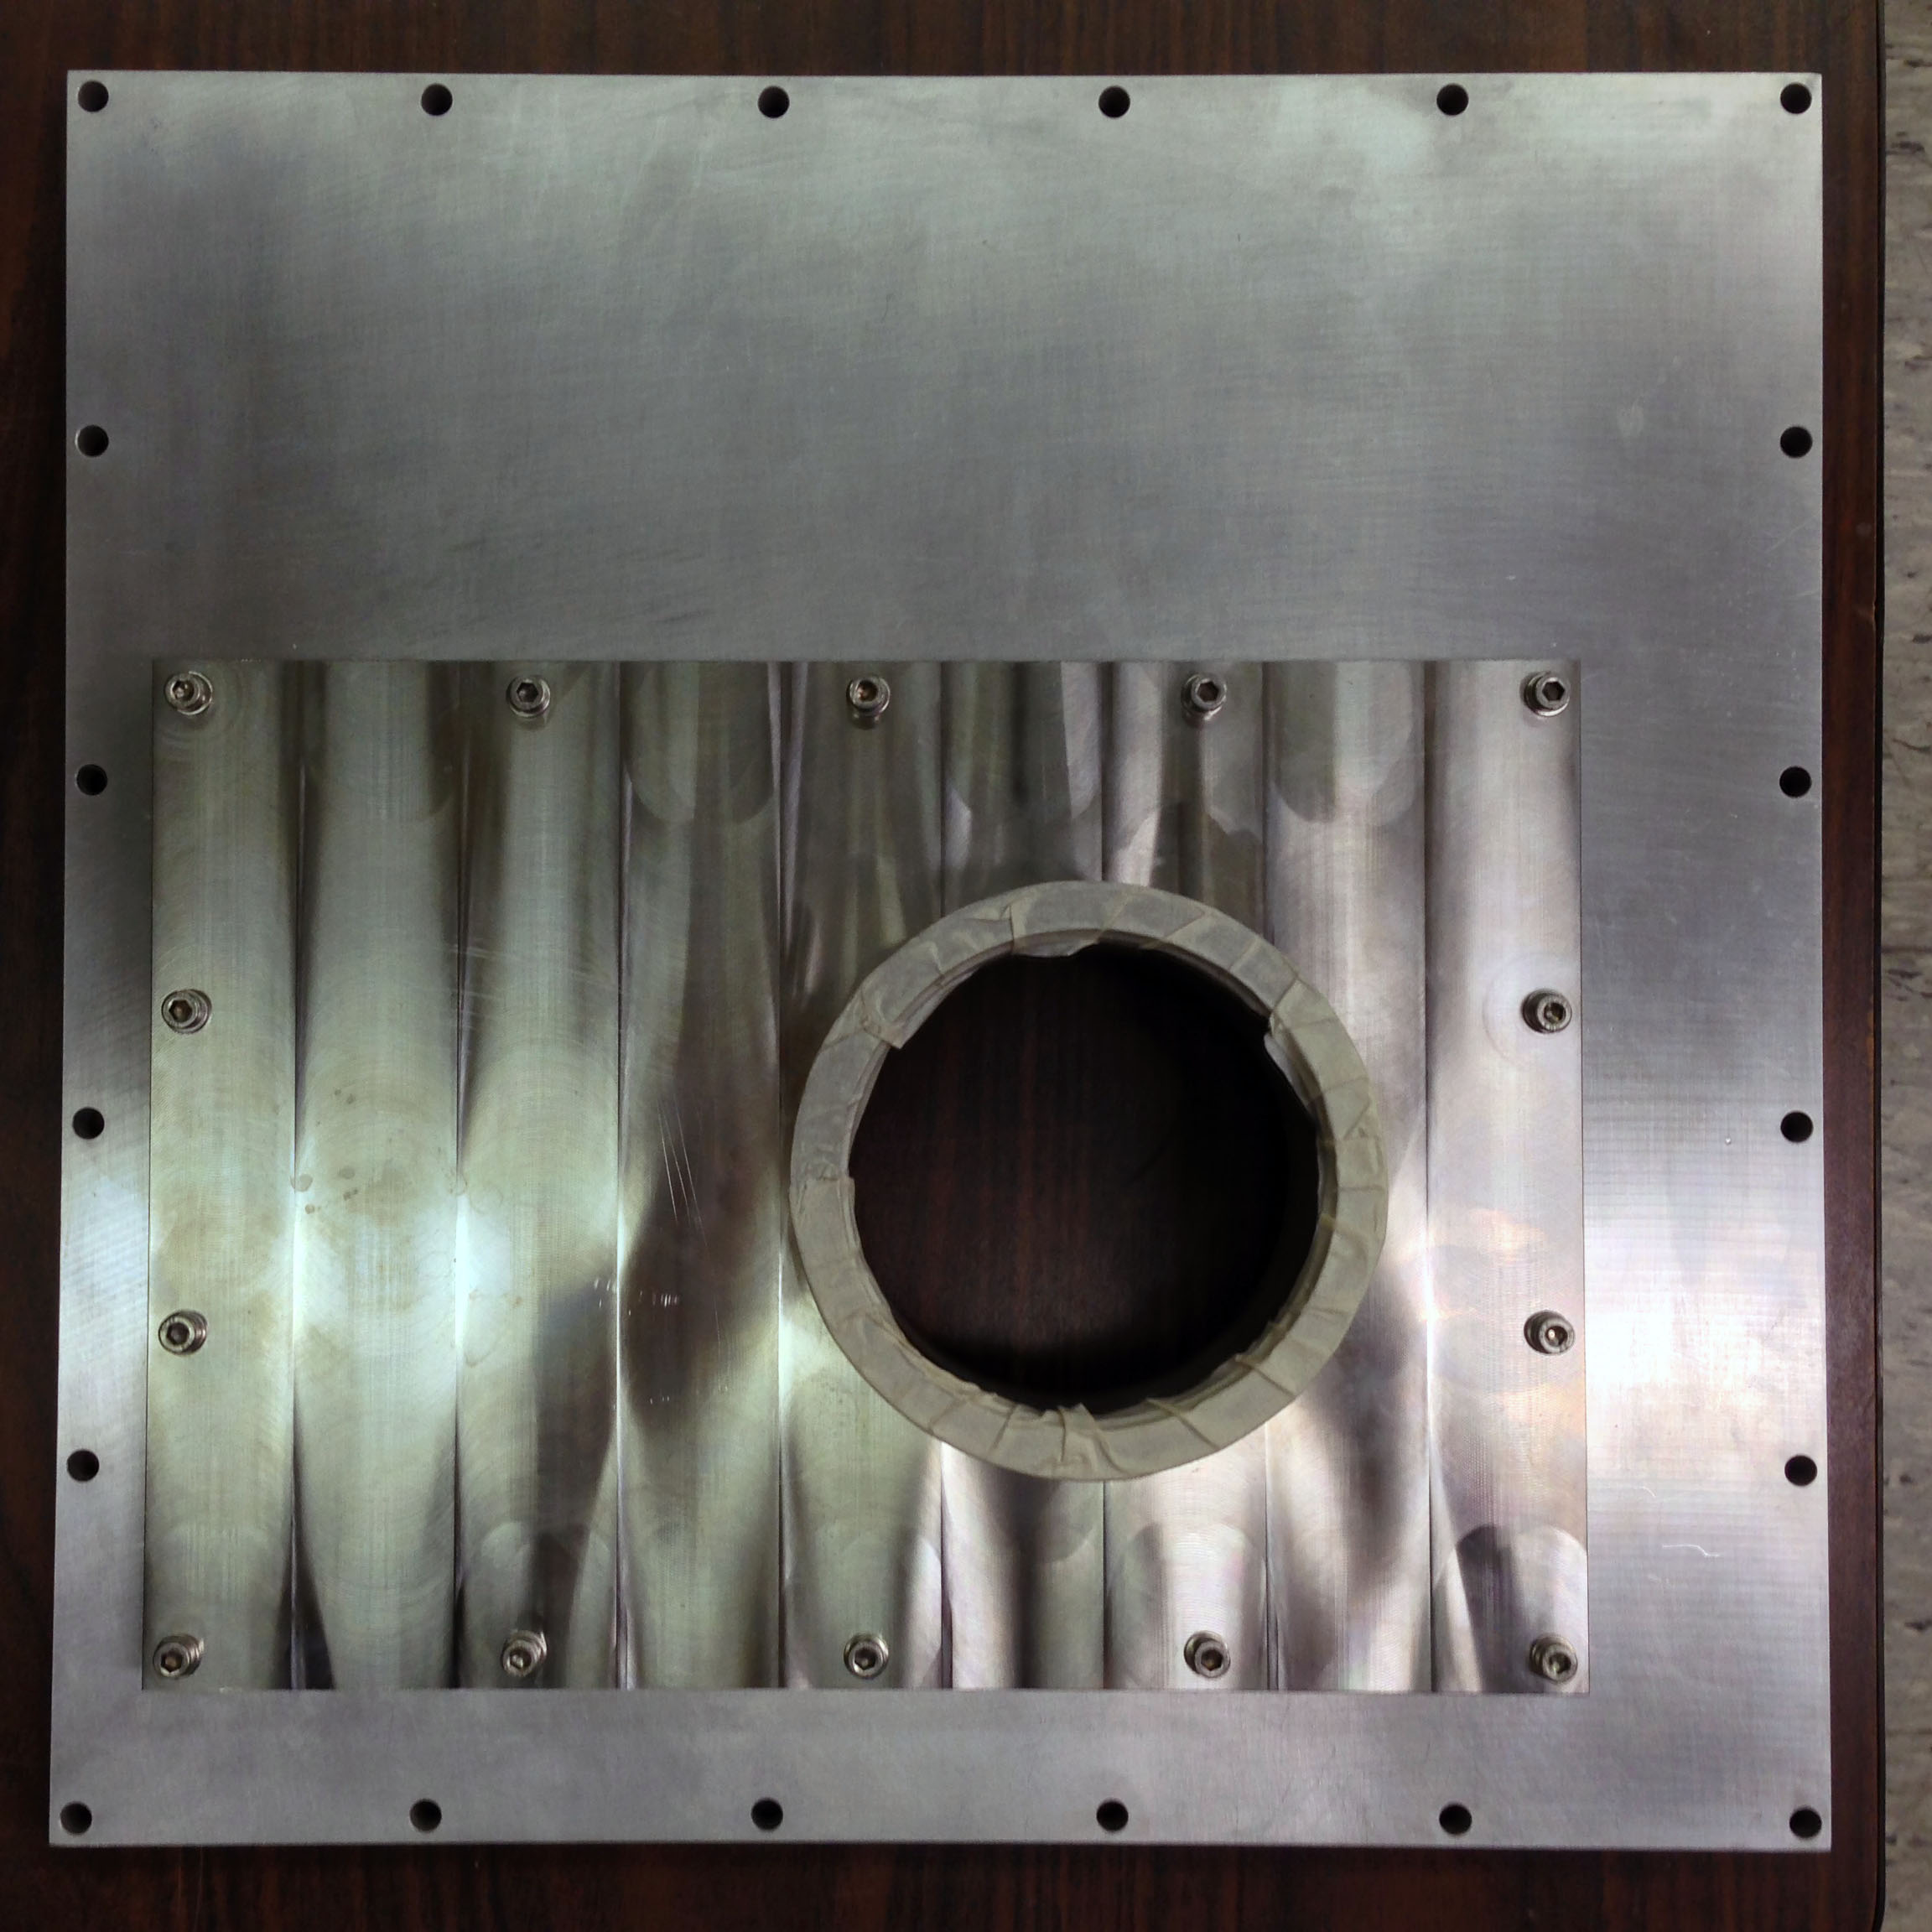
\includegraphics[width=0.48\textwidth, keepaspectratio]{IMG_0037c} \hspace{\fill}
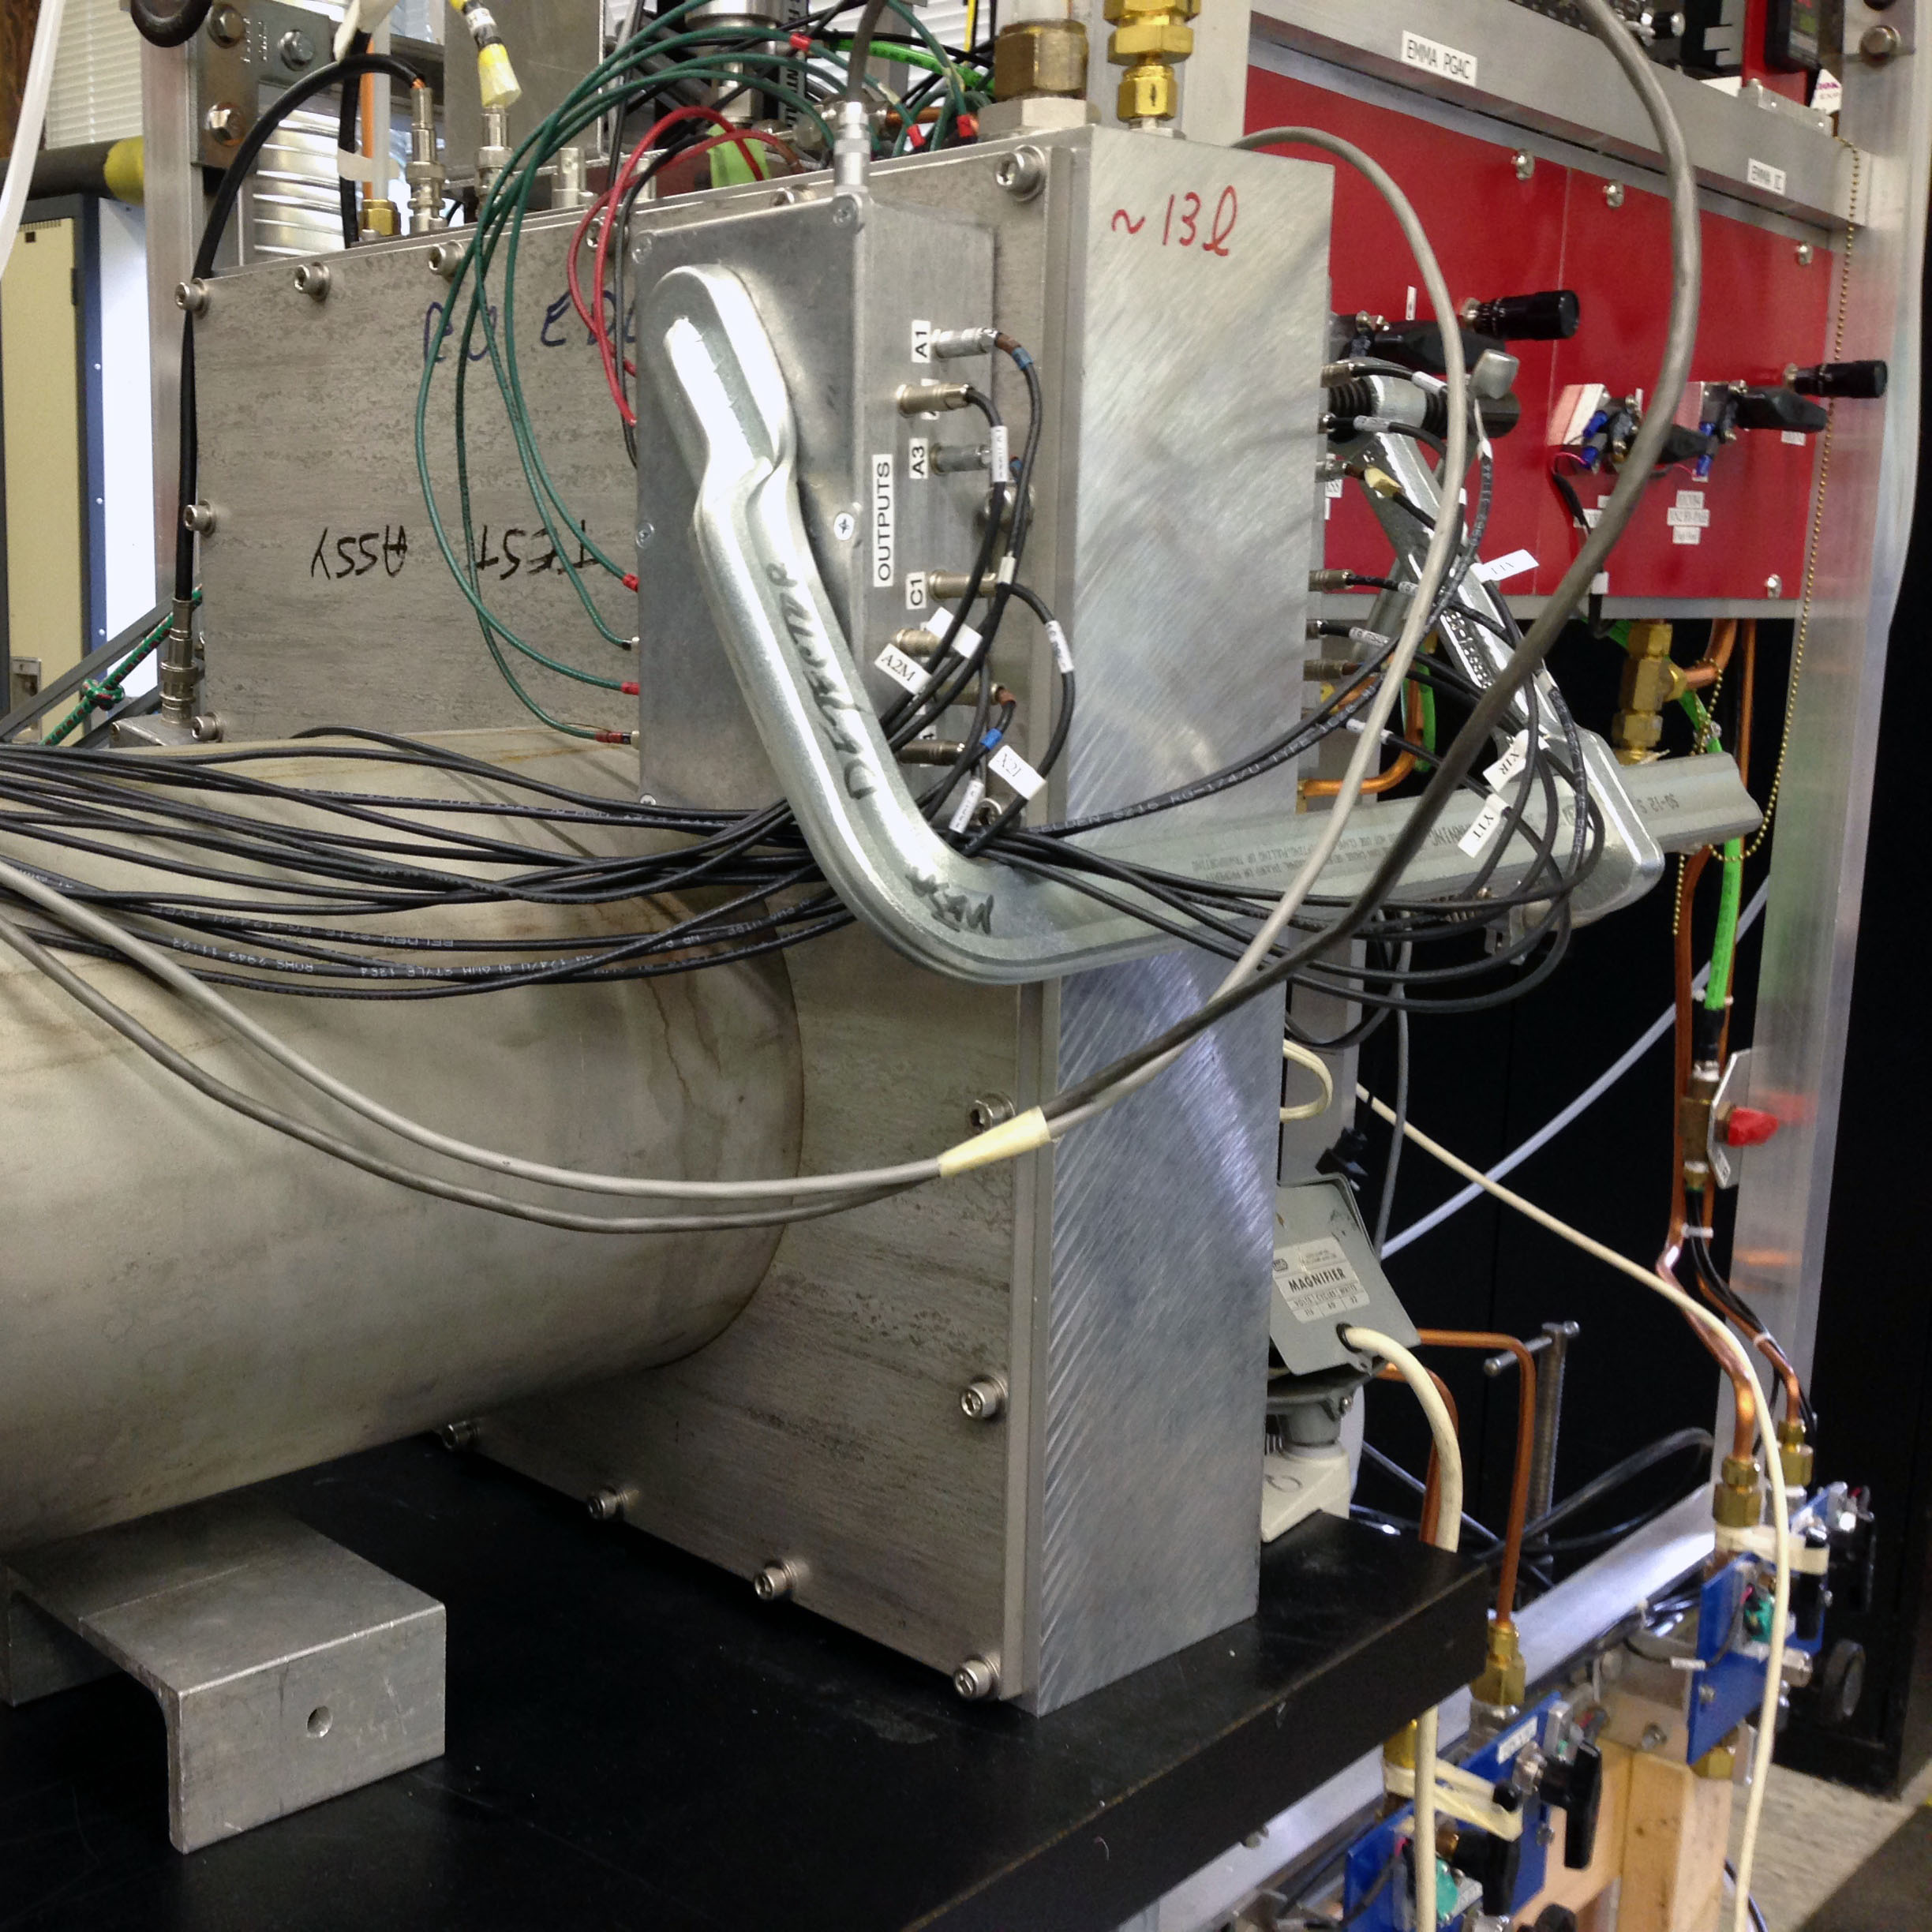
\includegraphics[width=0.48\textwidth, keepaspectratio]{IMG_0022c} \hspace{\fill}
\caption{(Left) The ``snout'' cover that will be used during the in-beam test to attach the PGAC box to the $0^\circ$ scattering chamber. (Right) The PGAC box and the gas-handing system during bench tests in the Detector Development Lab.}%
\label{photos}%
\end{figure}

\subsubsection{Electrical}
Beam scattered into the gas volume of the detector will cause ionization that will be accelerated by the %high
 voltages applied to the electrodes and multiplied by the gas into an ion avalanche.
The  voltage applied to the anode and cathode depend on the operating pressure of the detector.  At 4\,Torr, the voltage difference between the anode and cathode is typically 550\,V.  The anode is held at a positive voltage, 470\,V at 4\,Torr.  The two cathodes are held at a relatively small negative voltage, -80\,V at 4\,Torr.  The negative voltage on the cathodes is used to produce a potential difference between the cathodes and the walls of the chamber, which are at ground potential, in order to prevent the detection of ionization from outside of the active region.  

For each event, seven signals are output by each PGAC. Each cathode forms a delay line with 2.5\,ns added between adjacent cathode wires.  Signals are read from each end of the cathode with the position derived from the difference in time between the signals.  One cathode measures positions in the $x$-direction, the other measures positions in the $y$-direction, for a total of four cathode signals.
The anode is divided into three sections to reduce the capacitance of the detector and improve timing performance.  The anode signal is the characteristic timing signal of the PGAC.% and it 

All seven signals from the PGAC pass through a  %NIM mounted
pre-amplifier mounted to the chamber.  The pre-amp signals are further amplified using linear fast timing amplifiers.  The amplified signals are entered into a leading-edge discriminator to produce logic signals.  All seven logic signals are read into the acquisition system using a time-to-digital converter (TDC).  %boosts these signals
 %and the rise of the signals will be recorded with high time precision on a CAEN desktop digitizer. The digitizer must be triggered.
The logical OR of the anode signals is used to generate the trigger for the data acquisition system.%  This signal is fed into a fast leading-edge discriminator NIM module which provides the fast trigger to acquisition system.  


\subsection{Gas Handing System}
The newly-built EMMA gas handling system (GHS) will be used for the PGAC detector tests.
The gas handling system is designed to provide a stable flow of isobutane gas to the EMMA PGAC.  The hazards related to isobutane are discussed in \S\,\ref{flame}. The nominal volumetric flow rate is Q=60\,cc/min with Q$_\textrm{min}=20$ and Q$_\textrm{max}=100$.
The gas handling system must also maintain a constant set pressure  in the PGAC volume. The nominal operating pressure of the PGAC is 4--6\,Torr.
A schematic diagram of the vacuum and gas handling system  is shown in Fig.~\ref{diagram}. 
The primary design considerations for the EMMA PGAC GHS are to:

\begin{itemize}
\setlength{\itemsep}{0pt}
\setlength{\parskip}{0pt}
\setlength{\parsep}{0pt}
	\item Provide a stable operating pressure in the PGAC box
	\item Prevent a rupture of the thin PGAC window due to differential pressure during normal operations and during pumping and venting procedures
	\item Avoid flammable mixtures of air and isobutane
	\item Avoid the ignition of any flammable mixtures formed
	\item Protect the beam line vacuum from any rupture of the PGAC window
\end{itemize}

Isobutane is supplied from cylinders in the ISAC Gas Handling Building. The maximum flow into atmospheric pressure in the ISAC-II area is limited to 250\,cc/min by a low-pressure regulator feeding gas through a pre-set needle valve. The air-actuated valve \texttt{VA1} on the supply line 
is used to isolate the PGAC from the gas system when certain pressure interlocks are tripped and during pump-out and venting procedures.  On the  exhaust line, the PGAC is isolated by turning off pump \texttt{PU1} which automatically closes the pump valve.
\hyphenation{pro-por-tion-al}
Pressure control is provided by absolute pressure transducer \texttt{PA1}, flow controller \texttt{FC1} and the PID (proportional-integral-differential) controller. The PGAC pressure measured by \texttt{PA1} is input to the PID, which then outputs a signal to adjust flow through \texttt{FC1} such that the PID set-point pressure is maintained. %The flow out of the chamber is set by adjusting needle valve \texttt{VN1}.
 Differential pressure transducer \texttt{PD1} measures the pressure between the PGAC and the scattering chamber, e.g., the pressure across the PGAC window.% and is used to trigger interlocks if the differential pressure (in either direction) across the window exceeds threshold levels either during normal operation, or during filling and venting procedures.

Control of the flow of isobutane out of the PGAC chamber is  provided by precision needle valve \texttt{VN2} on the exhaust line upstream of scroll pump \texttt{PU1}. Ball valve \texttt{VB2} provides a large orifice bypass around \texttt{VN1} to allow efficient pumping to \texttt{VB6} for leak tests, and to allow efficient evacuation of isobutane from the PGAC prior to venting the system with air.

%Air-actuated valve \texttt{VA2} connects the PGAC volume to the diagnostic box during pump-out and venting procedures. \texttt{VA2} can also be forced open by a differential-pressure interlock to prevent destruction of the PGAC window from large differential pressure. This interlock only occurs, if other interlocks which are triggered at lower differential pressure have failed to remedy the situation. An interlock prevents \texttt{VA2} from being open if either or both of the gate valves \texttt{SEBT2IV2} and \texttt{SEBT2IV3} are open.

%\begin{landscape}
%\centering
%\vspace*{\fill}
\begin{figure}[t]
%\vspace*{-1in}
%\centering
\centerline{
\includegraphics[width=\columnwidth]{EMMA_ISAC1_GHS_1%
%logic_v6
}
}
\caption{Schematic diagram of the gas handling system and vacuum system for the EMMA PGAC commisioning experiment. Items labeled with the prefix \texttt{HEBT:} are controlled by EPICS.
%Devices shown above the diagnostic box are all gas system devices. Devices shown below the diagnostic box are all normal vacuum system devices in the HEBT beam line.
%Modifications to the existing gas system will be required and are indicated in blue.
}
\label{diagram}
\end{figure}
%\vspace*{\stretch{1}}
%\vfill
%\end{landscape}

Gas will be supplied from the ISAC gas shack through stainless steel flammable-gas lines where the
flow rate of the line is limited to 250\,cc/min into atmosphere. The gas exhaust from the
PGAC box will be pumped through roughing pump \texttt{PU1}, separate from the HEBT vacuum system, that will evacuate the detector gas through a gas exhaust line back to the gas shack.
The presence of the 2\,$\mu$m-thick Mylar window at the entrance of the PGAC box requires bypass valve \texttt{VB4}
to maintain a differential pressure within $\pm 4$\,Torr between the volume of the PGAC box and the volume of  the 0$^\circ$ scattering chamber
during pumping and venting procedures.

\subsection{Status}
\label{det_status}
The EMMA PGAC detector has been designed, built and tested by the TRIUMF Detector Development group.  The current phase of commissioning utilizes in-beam testing to commission the detector for in-beam use. % and is ready for beam tests for the next part of the commissioning procedure.
\subsubsection{Updates}
The current in-beam tests are a continuation of the in-beam tests performed in April 2014.
The tests will utilize the same interlocks and safety systems implemented on the HEBT beam line that were developed for the previous PGAC detector tests in April 2014~\cite{old_safety}. Following the recommendations of the safety review of the previous tests \cite{old_review}, the following additions have been made since the publication of the previous safety report. An interlock has been installed on the 110\,VAC power for the NIM crate used for the HV power supplies. All polyethylene tubing has been replaced with metal tubing. 
No further additions or adjustments to the safety systems have been made.
The improvements in the electronics setup and in the beam mask will %In-beam testing will also
 allow a more thorough examination of the position resolution and the particle trajectory reconstruction capacity of the detector system. % and maximum incident particle rate.

%test of the York PGAC.
%  In addition, 
%%\begin{enumerate}
%%\setlength{\itemsep}{0pt}
%%\setlength{\parskip}{0pt}
%%\setlength{\parsep}{0pt}
%%\item Convectron gauge \texttt{HEBT:CG19} has been connected to EPICS.
%%\item Needle valve \texttt{MVV19} has been installed downstream of valve \texttt{HEBT:VV19} to control the vent rate and protect the
%%PGAC window.
%%\item Interlock valve \texttt{VA1} has been installed.
%%\item A flammable gas sensor has been installed, commissioned, and calibrated in the experimental area.
%%\item The Controls group has provided a ``digital out'' port for valve \texttt{VA1},
%%a ``digital out'' port for the HV interlock, and an ``analogue in'' port for \texttt{FC1} flow signal.
%%\end{enumerate}
%the following hardware changes must be made:
%\begin{enumerate}
%\setlength{\itemsep}{0pt}
%\setlength{\parskip}{0pt}
%\setlength{\parsep}{0pt}
%\item In order to use HV power supplies other than the Iseg modules (which have higher-than-desirable  current limits, but already accept an interlock signal from EPICS), a HV interlock must be installed on the 110\,VAC power to the NIM crate.  Failing that, the Iseg HV power supplies will be used.
%%, e.g. a commercially available 110\,VAC switch on the HV power supplies  NIM crate supply line.
%\item Tubing between \texttt{FC1} and the PGAC box; the PGAC box, valve \texttt{VB4}, and the scattering chamber; and between
%the gas supply panel and \texttt{PU1} should all be copper or stainless steel.
%\item (Optional) A mask may be fabricated and installed to characterize the position sensitivity of the PGAC.
%\end{enumerate}
\subsubsection{Bench Tests}
The PGAC is designed to be operated with heavy ion beams.  The ionization potential of $\alpha$-decay sources, such as the $^{241}$Am source used in the bench tests,  is insufficient to adequately test the performance of the detector.  For example, with the detector optimized for $\alpha$ particles at 5\,Torr, the signal-to-ratio is %3--4:1
2.7:1  for the cathode, 10.9:1 for the andode,
 and the timing resolution is 1.8\,ns~FWHM.  %The jitter induced by the slow rise times of the weak signals
The ionization from the scattered $^{16}$O beam will be a factor of 12.1 greater than the ionization from the $\alpha$ particles from $^{241}$Am. The robust signals produced by the $^{16}$O will improve the timing resolution by about a factor of 3 and provide a more accurate characterization of the detector.

During testing with the $\alpha$ source, no Mylar window was used on the entrance of the PGAC box.  A 0.9\,$\mu$m-thick window was stress tested and shown to burst at a differential pressure 24\,Torr.  The Mylar window is not supported by wires, therefore the burst pressure is the same in both directions.  During the in-beam testing, a  2.0\,$\mu$m-thick Mylar window will be used.  
The burst pressure of the 2.0\,$\mu$m-thick Mylar window was measured to be 57\,Torr (which is consistent with a linear relationship between window thickness and burst pressure).
%The pressure tolerance of the  2.0\,$\mu$m-thick window is estimated to be 100--200\,Torr.  However, the burst pressure of a window of that thickness has not yet been tested. 



